\documentclass{beamer}

\usepackage{mpemath}
\usepackage{subcaption}
\usepackage[normalem]{ulem}
\usepackage{amsmath}
\usepackage{amssymb}
\usepackage{mathtools}
%\usepackage{pgf}
%\usepackage{pgfplots}
%\usepackage{tikz}
\usepackage{booktabs}
\usepackage{siunitx}
\usepackage{natbib}
\usepackage{tabularx}
\usepackage{multirow}
\usepackage{amsmath}
\usepackage{mathtools}
\usepackage{amssymb}
\usepackage{bbm}
\usepackage[dvipsnames]{xcolor} % Saved my life during a conference once


%\usetikzlibrary{arrows,automata,backgrounds,positioning,decorations,intersections,matrix}

% *** Styles ***
\usetheme{Singapore}
\setbeamertemplate{navigation symbols}{}
% \usetheme[progressbar=frametitle]{metropolis}
% \usecolortheme{dolphin}
%\useinnertheme{circles}
%\usecolortheme{rose}
%\setbeamercovered{transparent}
\setbeamercovered{invisible}
\usefonttheme{professionalfonts}
%\usefonttheme[onlymath]{serif}
\setbeamertemplate{footline}[frame number]

\title{Reinforcement Learning and Optimal Control}
\author{Gersi Doko}
\institute{Department of Computer Science \\ University of New Hampshire}
\date{}

\AtBeginSection[]{
	\begin{frame}
          \vfill
	\centering
	% \usebeamerfont{title}
        {\huge\bf \insertsectionhead}%
	\vfill
\end{frame}
}

\begin{document}

\frame{\titlepage}

\section*{Intro}

\begin{frame}
\frametitle{What do we do?}
	\begin{itemize}
		\item Solve sequential decision making problems
		\vfill
		\item Given a model of the environment
		\vfill
	        \item In recent work we do not assume a goal/reward function
	\end{itemize}
\end{frame}

\section*{ROIL}

\begin{frame}
	\frametitle{ROIL}
	\emph{Robust} method for \emph{off-policy} Inverse Reinforcement Learning (IRL)

	\vfill
	\emph{Motivation}
	\begin{itemize}
	  \item Need methods that learn from human data
	  \item Methods need to generalize to unseen data
	\end{itemize}
\end{frame}

\begin{frame}
	\[ \textcolor{red}{\min_{u^\pi \in \mathcal{U}}} \; \textcolor{ForestGreen}{\max_{u_e \in \Upsilon}} \; \textcolor{purple}{\max_{r \in \mathcal{R}}} \;return(\textcolor{ForestGreen}{u_e}, \textcolor{purple}{r}) - return(\textcolor{red}{u^\pi}, \textcolor{purple}{r})\]
  \vfill
  \begin{center}
	  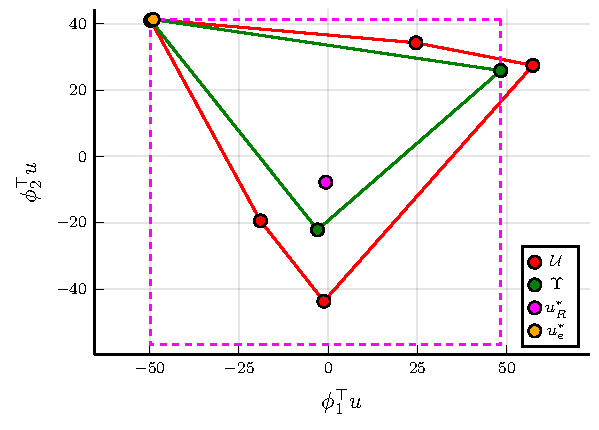
\includegraphics[width=0.95\textwidth, height=0.85\textheight]{../../pres_roil/plots/visual_solve_cheb.pdf}
  \end{center}
\end{frame}

\section*{Conclusion}

\begin{frame}
	\frametitle{Conclusion}
	\begin{itemize}
	  \item RL Group Meetings 
	  \item Thursday 2:00pm-3:30pm Kings N233
	  \vfill
	  \item Questions? Reach out! Gersi.Doko@unh.edu
	\end{itemize}
\end{frame}

\end{document} 
